\documentclass[conference]{IEEEtran}
\usepackage[T1]{fontenc}
\usepackage{cite}
\usepackage{amsmath,amssymb}
\usepackage{graphicx}
\usepackage{booktabs}
\usepackage{url}
\usepackage[hidelinks]{hyperref}
\newcommand{\SA}{\mathrm{SA}}
\newcommand{\GEQO}{\mathrm{GEQO}}
\begin{document}
\title{Reliability of Stochastic Join-Order Optimization:\\Measuring Regression Risk and Evaluating Safeguards\\in Quantum-Augmented Query Planning}
\author{\IEEEauthorblockN{Abhishek Humagain}
\IEEEauthorblockA{First research draft --- November 19, 2026}}
\maketitle
\begin{abstract}
Stochastic join-order search can produce different physical plans for the same
query, yet improved model cost or average execution time alone does not establish
reliable database performance. We present a reproducible evaluation pipeline that
separates optimizer draws, plan-enforcement failures, physical-plan variability,
and execution measurements. An exploratory CPU pilot applies simulated annealing
(SA) to a published quantum-optimization binary model and compares it with seeded
PostgreSQL genetic query optimization (GEQO) on twelve selected Join Order
Benchmark templates. Across 720 optimizer trials, 715 proposals pass verification;
485 distinct physical plans induce 2,425 scheduled execution slots. The pipeline
retains timeouts and unavailable comparisons rather than replacing them with
numeric timeout caps. A post-hoc clock audit flags 27 measured repeats across 23
plans, and baseline variability limits performance interpretation. After the
quality screen, descriptive identification bounds for profiled slowdown exceeding
1.25 times the baseline are 48.6--86.7\% for SA and 25.0--44.2\% for GEQO.
A separate 360-slot baseline calibration detects no clock discrepancies but retains
substantial timing variability. A simple estimated-cost guard rejects all SA
proposals, illustrating why fallback
frequency and useful optimization must be evaluated together. These results are
an engineering pilot, not a quantum-hardware evaluation, a full QDBO reproduction,
or evidence of population-level runtime superiority.
\end{abstract}
\begin{IEEEkeywords}
query optimization, join ordering, stochastic optimization, regression risk,
quantum-inspired optimization, reproducibility
\end{IEEEkeywords}

\section{Introduction}
Join ordering exposes a database optimizer to a large search space, imperfect
cardinality estimates, and competing physical execution choices. The Join Order
Benchmark (JOB) demonstrates that estimation and enumeration can both matter
substantially for real multi-join queries~\cite{leis2015job}. Quantum and
quantum-inspired approaches provide additional ways to search mathematical
encodings of this problem~\cite{schonberger2023digital,liu2025q2o,liu2026qdbo}.
Their practical value depends on the complete path from an optimizer output to a
verified database plan and its execution cost.

A low model objective does not guarantee a fast physical plan. Repeating a
stochastic optimizer can change the decoded order, while PostgreSQL still chooses
scan methods, join implementations, and other physical operators. A requested
hint can also fail to enforce the intended tree. Finally, execution variation and
measurement instrumentation can obscure the difference between a search failure
and a measurement failure. Evaluating only successful or improved outputs hides
these distinctions.

We investigate three questions. \emph{RQ1:} How variable are verified physical
plans under fixed optimizer inputs? \emph{RQ2:} What fraction of planned optimizer
outputs can be compared with the default plan, and what descriptive regression
risk remains when unknown outcomes are retained? \emph{RQ3:} Does an estimated-cost
fallback offer useful optimization, rather than simply selecting the default?

This draft makes three limited contributions. First, it describes an auditable
pipeline with durable trial records, directed-tree checks, plan deduplication,
and explicit timeout accounting. Second, it reports a completed twelve-template
CPU pilot and separates output variability from runtime coverage. Third, it
identifies measurement-validity and safeguard-utility issues that must be
resolved before a stronger experiment. We do not claim the first stability study
of quantum join ordering: prior work explicitly studies optimization
stability~\cite{shekar2026spiq}. We also make no claim of quantum advantage.

\section{Background and Related Work}
\subsection{Quantum and Quantum-Inspired Join Ordering}
Digital annealing work studies join-order encodings, probabilistic outputs, and
readout methods, including classical SA comparisons~\cite{schonberger2023digital}.
Q2O integrates hybrid optimization with PostgreSQL through join-order
hints~\cite{liu2025q2o}. QDBO introduces mapping and iterative correction for
low-level quantum sampling and integrates the optimizer with a database
system~\cite{liu2026qdbo}. Our pilot uses its published binary quadratic model
(BQM) builder and decoder with CPU SA. It omits quantum embedding, hardware
sampling, and the full iterative correction procedure. Consequently, our results
evaluate this adaptation, not the reported QDBO system.

Structured initialization for gate-based join ordering studies stability and
solution-quality distributions in small simulation-based
instances~\cite{shekar2026spiq}. Hybrid QUBO research also investigates
selectivity and connected-order constraints~\cite{nayak2026hybridjournal}.
Repeated outputs, initialization robustness, and connectivity repair are therefore
established research topics. Our working focus is the downstream accounting of
verified physical plans, unavailable database comparisons, and safeguard
utility; priority and completeness still require a broader literature review.

\subsection{Database Regressions and Safeguards}
Bao steers an existing optimizer with learned hint choices and addresses practical
performance, including tail behavior~\cite{marcus2021bao}. Eraser uses risk
filtering and prediction-quality assessment to mitigate learned-optimizer
regressions~\cite{weng2024eraser}. Conformal verification also studies checks and
violation handling for learned optimization~\cite{liu2025conformal}. These systems
motivate explicit regression evaluation, but our simple planner-cost comparison
is not a reproduction of their methods and provides no runtime guarantee.
Robust Predicate Transfer instead changes execution behavior to reduce sensitivity
to join order~\cite{zhao2025rpt}; our pipeline leaves the execution engine intact.

\section{Reliability Model and Metrics}
\subsection{Units and Plan Identity}
For query $q$, let $n_q$ denote the number of planned optimizer draws for one
method. A draw may yield a verified physical plan, an unenforced requested tree,
or another recorded failure. Each verified physical plan has a canonical
structural fingerprint. Repeated draws returning the same fingerprint count
separately in the optimizer output distribution but share execution measurements.
The baseline is PostgreSQL's default planning policy under the frozen settings.
A model objective, a PostgreSQL estimated cost, and an observed execution time are
distinct quantities throughout the analysis.

If $c_{qp}$ verified draws return physical plan $p$ and $v_q$ draws are verified,
pairwise plan disagreement is
\begin{equation}
 D_q=1-\frac{\sum_p c_{qp}(c_{qp}-1)}{v_q(v_q-1)},\qquad v_q>1.
\end{equation}
This is the fraction of ordered pairs of distinct verified draws with different
fingerprints. It is conditional on verification and is not an execution-noise
metric. We average $D_q$ across queries rather than interpreting draws from one
query as independent workload instances.

\subsection{Execution Coverage and Descriptive Risk}
Each eligible physical plan has five scheduled measured repetitions after a
warmup. A median is available only when all five measured repetitions succeed
and pass the timing-quality screen described in Section~\ref{sec:quality}.
Let $T_q(p)$ be this median and $b_q$ the baseline plan. The ratio
\begin{equation}
 r_{qi}=T_q(p_{qi})/T_q(b_q)
\end{equation}
is unknown if either median or the verified candidate is unavailable. For a
threshold $\tau$, define $s_q(\tau)$ as the number of known ratios greater than
$\tau$, and $u_q$ as the number of unknown ratios among all $n_q$ planned draws.
Then
\begin{equation}
 L_q(\tau)=\frac{s_q(\tau)}{n_q},\qquad
 U_q(\tau)=\frac{s_q(\tau)+u_q}{n_q}.
\end{equation}
Averaging these endpoints equally across queries gives descriptive identification
bounds over the observed pilot. They are not confidence intervals, and they do
not address timing noise in known ratios. We use $\tau\in\{1.10,1.25,2.00\}$
as descriptive sensitivity points, not established practical-effect thresholds.

A timeout is a censored attempt, not a successful 60-second execution. We retain
it and mark the remaining repetitions of that plan as unrun. A failed baseline
makes every candidate-to-baseline ratio for that query unknown. This conservative
accounting does not infer additional slowdown events from partial observations.

\subsection{Offline Estimated-Cost Guard}
The guard falls back to $b_q$ if candidate verification fails or if its estimated
PostgreSQL Total Cost exceeds the cached baseline estimate. Otherwise it selects
the candidate. The diagnostic reuses measured plan medians; it does not actually
replay a guarded request. In particular, a guard comparison measured in
microseconds is not the end-to-end cost of optimization, validation, fallback
planning, and execution. We report fallback frequency alongside risk coverage
because an always-fallback policy cannot establish useful optimization.

\section{Experimental Method}
\subsection{Workload, Environment, and Controls}
The workload contains twelve distinct JOB templates, with one variant per template
and four selected templates in each of three relation-count strata. Selection was
fixed before runtime collection and additionally covers graph and self-join
features. This is a coverage sample, not a probability sample of all 113 JOB
queries. Selected instances have four to seventeen relations (Table~\ref{tab:queries}).
Canonical IMDB data contain 21 tables and 74,190,187 rows. We use the canonical
primary-key and foreign-key-column indexes, without adding foreign-key
constraints, and retain a fingerprint of the analyzed statistics snapshot.

The host is an Apple M4 with ten CPU cores and 16~GiB of memory, running macOS
26.2. The isolated PostgreSQL 18.3 cluster loads pg\_hint\_plan 1.8.1 per session.
Execution uses 4~MB \texttt{work\_mem}, disabled parallel execution and JIT, and a
60-second statement timeout. Sessions are read-only. No QPU or commercial hybrid
service is used.

\subsection{Optimizer Draws and Enforcement}
For each query, PostgreSQL estimates filtered base cardinalities and pairwise
predicate factors. These inputs and the resulting BQM are fixed across thirty
SA seeds. Each draw uses ten reads and 200 sweeps, selects the lowest-energy read,
and applies the unchanged upstream decoder, including its postprocessing. The
raw membership-validity check tests relation-count and nesting constraints; it
is not a check of every auxiliary encoding constraint.

Thirty GEQO trials per query force \texttt{geqo\_threshold=2}, with seeds
$(i+1)/31$ for $i=0,\ldots,29$, and effort/pool-size/generation settings 5/0/0.
The default baseline uses threshold 12 and seed zero. GEQO is PostgreSQL's genetic
search mechanism~\cite{postgres18geqo}. Equal draw counts do not equalize compute
budgets, plan spaces, or objective functions.

SA orders are passed through directed nested \texttt{Leading} hints, with GEQO
disabled for that planning step. Directed hints fix outer/inner orientation; the
pinned QDBO helper instead emits a flat list that leaves these choices free.
This restriction is a material adaptation requiring a future ablation. Structural
tree comparison, rather than a hint-status message, determines whether a request
was enforced. Hint-enabled and hint-disabled controls are collected. Every
successful timed execution is checked again against the expected tree, when
specified, and the preflight physical-plan fingerprint.

\subsection{Scheduling, Durability, and Measurement}
All 720 optimizer trials finish before any execution timing is observed. For each
query, verified candidate and baseline fingerprints are deduplicated. Every
eligible distinct plan receives one warmup, followed by five deterministic
randomized blocks containing the eligible candidates and baseline. A warmup is
a policy, not a guarantee that the working set fits in cache. After a timeout or
other execution failure, the remaining scheduled slots are explicitly marked as
unrun. Finished successes and failures are not redrawn on resume.

A single-owner SQLite ledger durably records task state and attempts. A clean
checkpoint and subsequent resume preserve the first eight completed records.
After full completion, a no-op resume preserves all 3,678 task payloads. The
measurement source revision is recorded separately from later analysis and
recovery hardening. Postrun checks confirm that installed package versions and
upstream tracked Python sources match the initial environment; the historical
runner did not enforce these checks on each resume.

Timing uses EXPLAIN ANALYZE with buffer statistics and JSON output, and default
node-level \texttt{TIMING ON}. PostgreSQL documents that repeated node clock reads
can add substantial profiling overhead and that ordinary query execution can
therefore be faster~\cite{postgres18explain}. We call these values \emph{profiled
executor times}, not application latency. A separate baseline-only TIMING OFF/plain-query calibration is reported in
Section~\ref{sec:calibration}; it does not replace the candidate profiles.

\subsection{Post-Hoc Timing Quality Screen}\label{sec:quality}
After the run, some successful PostgreSQL profiles exceed the enclosing client
monotonic duration by tens of seconds or minutes. The discrepancy is consistent
with system sleep during overnight execution, but an OS sleep trace was not
collected and the cause is not proven. A statement timeout does not validate
such recorded durations.

We explicitly introduce a \emph{post-hoc} screen: if any successful measured
repeat has server execution time greater than client elapsed time plus 1,000~ms,
its entire plan median becomes unavailable. We neither substitute the client
clock nor form a median from fewer repeats. All raw observations and unscreened
five-success medians are retained. The screen flags 27 measured repeats across
23 plans: one repeat each in \texttt{13a} and \texttt{25a}, and 25 in \texttt{28a}.
Five \texttt{28a} warmups also exhibit the discrepancy; these are disclosed but
do not alter historical eligibility. Across both phases, the detected excesses
range from about 58 seconds to 59 minutes, well above the chosen tolerance.
The screen does not establish that other timings are unaffected.

\begin{figure*}[t]
\centering
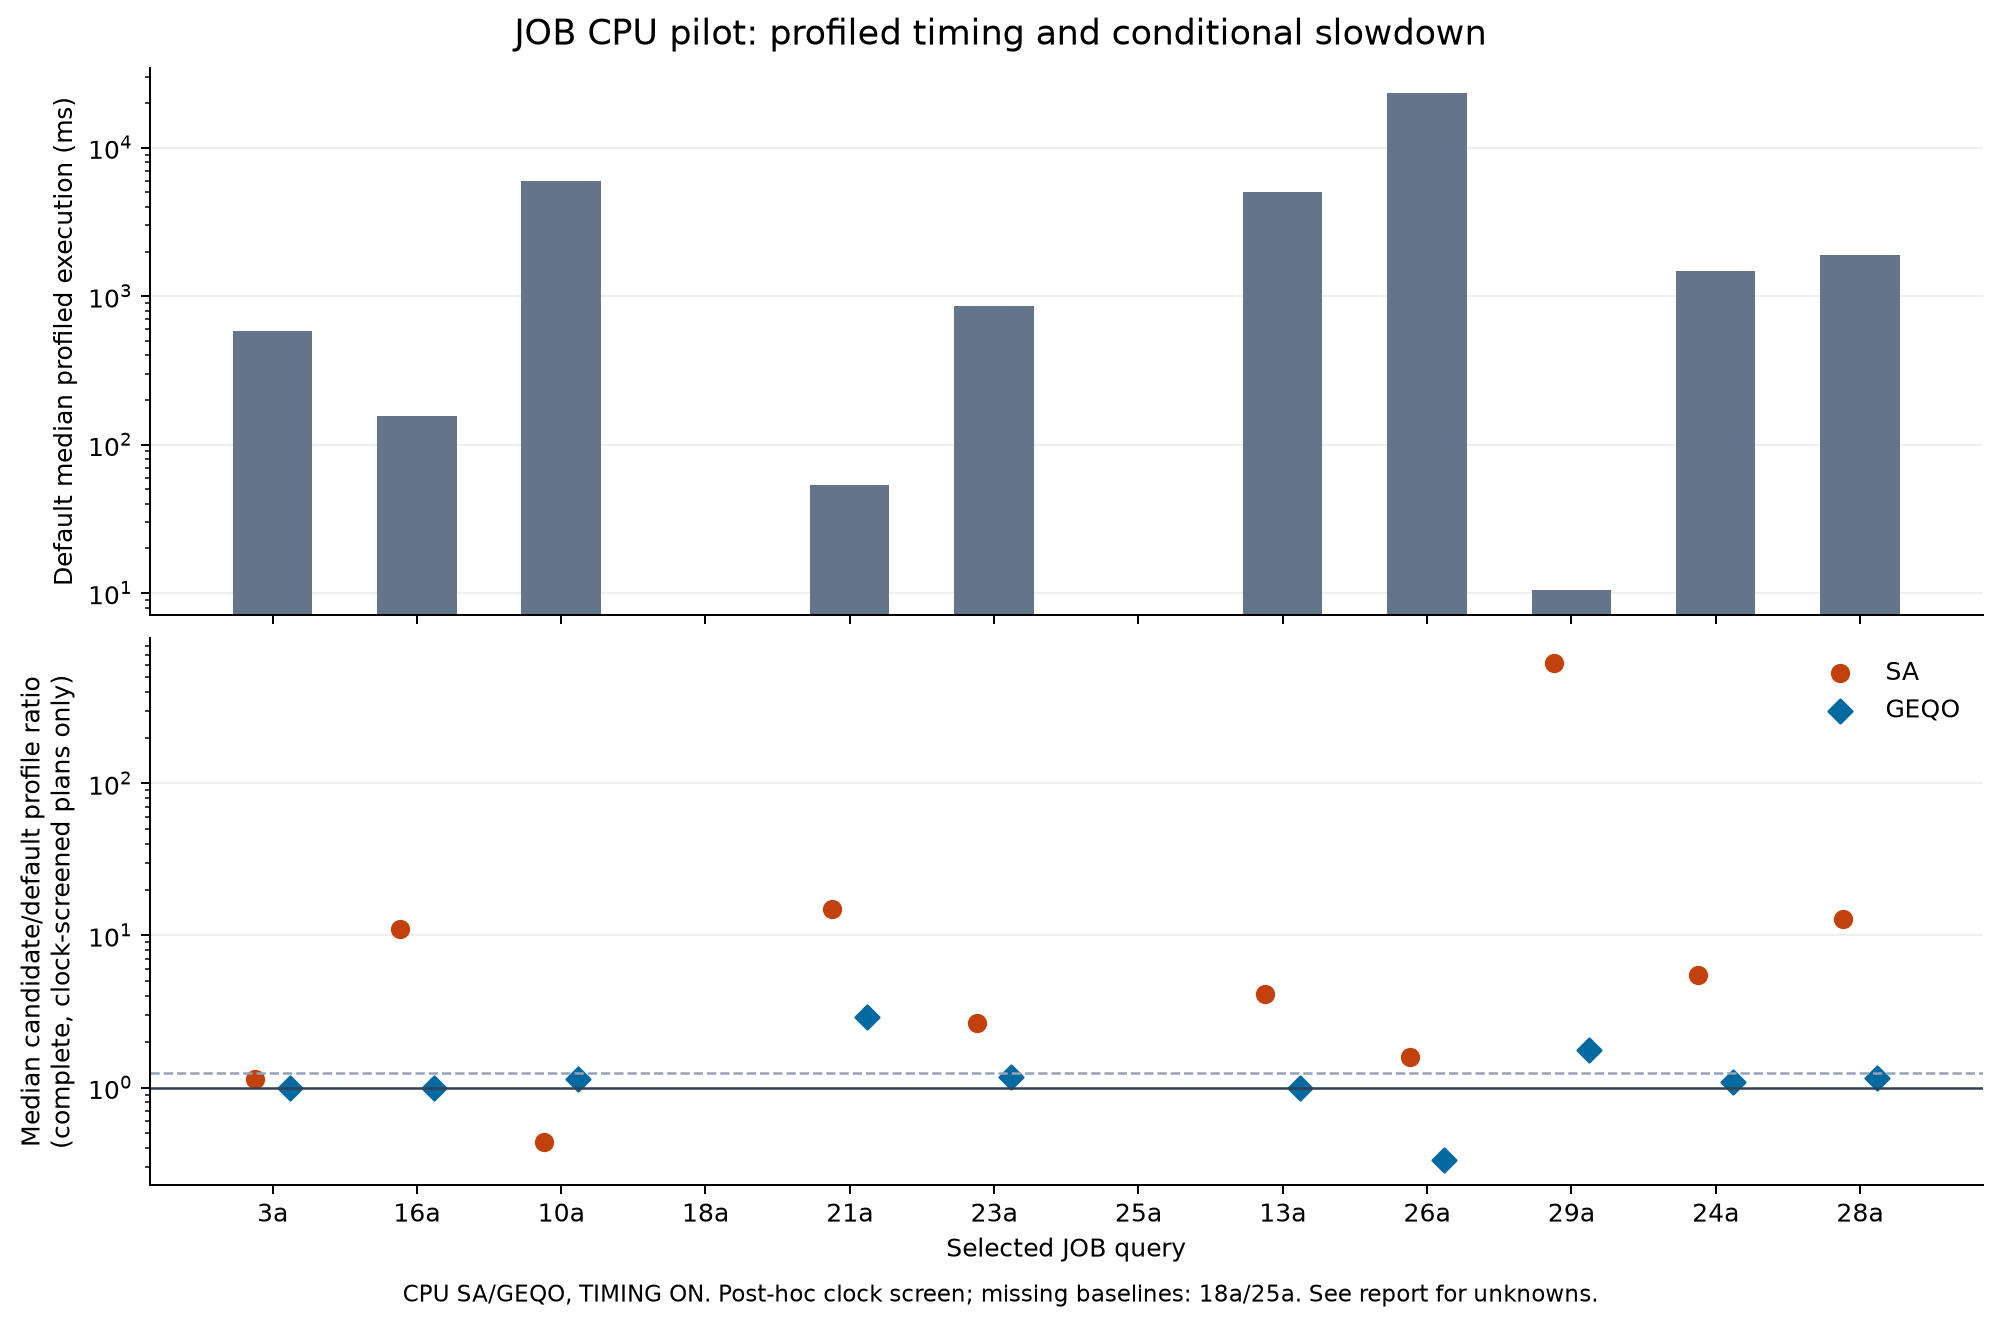
\includegraphics[width=.92\textwidth]{figures/pilot.png}
\caption{Exploratory CPU pilot. Top: default profiled median execution time.
Bottom: per-query median candidate/default ratio over available optimizer draws.
Each candidate plan must have five successful, clock-screened repeats. Missing
baselines make \texttt{18a}/\texttt{25a} unavailable. Complete-only summaries can
hide substantial unknown coverage; interpret them with Table~\ref{tab:queries}.
No confidence intervals or quantum-hardware results are shown.}
\label{fig:pilot}
\end{figure*}

\section{Pilot Results}
\subsection{Accounting and Physical-Plan Variability}
All 720 planned optimizer trials are recorded: 355/360 SA and 360/360 GEQO
proposals pass verification. Five SA requests fail directed-tree enforcement and
remain in trial denominators. Across queries there are 485 distinct physical
plans including baselines. The schedule contains 2,425 measured slots: 2,042
successful executions, 14 timeouts, and 369 explicitly unrun slots after timeout.
Warmups comprise 418 successes and 67 timeouts. All successful measured executions
pass the structural checks; this does not certify their timing validity.

Mean per-query disagreement among verified draws is 0.971 for SA and 0.588 for
GEQO. Table~\ref{tab:queries} shows that GEQO returns one fingerprint on some
queries but many on others. High disagreement is not itself a defect: multiple
plans could have similar runtimes. Raw SA membership checks pass 206/360 draws.
Because upstream decoding can repair outputs and the check omits auxiliary
constraints, this count cannot be interpreted as a complete feasibility rate or
as the cause of runtime regressions.

\begin{table}[t]
\caption{Pilot coverage. Known ratios count planned draws with available
candidate and baseline medians after the post-hoc screen, out of 30 per method.
Dashes denote unavailable baseline measurements.}
\label{tab:queries}
\centering\scriptsize
\setlength{\tabcolsep}{3.0pt}
\begin{tabular}{@{}lrrrrrrr@{}}
\toprule
& & \multicolumn{2}{c}{Default profile} & \multicolumn{2}{c}{Distinct plans} & \multicolumn{2}{c}{Known ratios}\\
Query & Rel. & Median ms & CV & SA & GEQO & SA & GEQO\\
\midrule
3a & 4 & 586.38 & 0.48 & 5 & 1 & 30 & 30 \\
16a & 8 & 156.93 & 1.18 & 27 & 5 & 19 & 30 \\
10a & 7 & 5936.79 & 0.18 & 26 & 1 & 30 & 30 \\
18a & 7 & -- & -- & 27 & 1 & 0 & 0 \\
21a & 9 & 53.29 & 0.68 & 29 & 9 & 29 & 30 \\
23a & 11 & 856.67 & 0.60 & 30 & 16 & 30 & 30 \\
25a & 9 & -- & -- & 30 & 10 & 0 & 0 \\
13a & 9 & 5022.19 & 0.25 & 30 & 2 & 7 & 30 \\
26a & 12 & 23416.47 & 0.12 & 29 & 23 & 16 & 28 \\
29a & 17 & 10.53 & 1.16 & 30 & 30 & 28 & 30 \\
24a & 12 & 1469.64 & 0.84 & 30 & 27 & 30 & 30 \\
28a & 14 & 1883.70 & 0.36 & 30 & 29 & 4 & 23 \\
\bottomrule

\end{tabular}
\end{table}

\subsection{Regression Coverage and Noise}
The default plans for \texttt{18a} and \texttt{25a} time out, so no runtime ratio
is available for those queries. After the clock screen, 223/360 SA ratios and
291/360 GEQO ratios are available. The ten completed baselines have five-repeat
coefficients of variation ranging from 0.120 to 1.178. Such variation makes
small threshold crossings unstable; this pilot does not establish a practical
noise-adjusted regression threshold.

At $\tau=1.25$, SA has 175 confirmed slow draws and 137 unknowns, yielding
48.6--86.7\% bounds. GEQO has 90 confirmed slow draws and 69 unknowns, yielding
25.0--44.2\%. Table~\ref{tab:risk} reports the other descriptive thresholds.
These are bounds for the recorded profiled ratios under the stated screen,
not evidence that SA is generally less reliable or that solver randomness
caused the observed differences. Before screening, the corresponding arithmetic
bounds were 52.5--86.7\% and 26.4--43.6\%; those figures include timing-invalid
profiles. Figure~\ref{fig:pilot} summarizes the conditional per-query medians.

\begin{table}[t]
\caption{Query-weighted descriptive slowdown bounds (\%). Guard columns are
an offline diagnostic. Intervals retain unknown comparisons; they are not
confidence intervals.}
\label{tab:risk}
\centering\small
\begin{tabular}{@{}lrrr@{}}
\toprule
Method & Threshold $\tau$ & Unguarded & Offline guard\\
\midrule
CPU SA & 1.10 & 53.6--91.7 & 0.0--16.7 \\
CPU SA & 1.25 & 48.6--86.7 & 0.0--16.7 \\
CPU SA & 2.00 & 42.5--80.6 & 0.0--16.7 \\
GEQO & 1.10 & 35.3--54.4 & 15.0--32.8 \\
GEQO & 1.25 & 25.0--44.2 & 6.1--23.9 \\
GEQO & 2.00 & 12.8--31.9 & 1.9--19.7 \\
\bottomrule

\end{tabular}
\end{table}



\subsection{Fallback Frequency and Optimizer Overhead}
The estimated-cost guard rejects all 360 SA proposals and 134/360 GEQO proposals.
For SA, the diagnostic therefore reduces to always selecting the default. Its
zero confirmed slowdowns on measurable baselines is expected from that policy,
not evidence of a useful optimizer improvement. Its upper bound remains 16.7\%
because two baseline medians are unavailable. A real safeguard evaluation must
measure useful accepted proposals, fallback frequency, and full request latency.

Median SA optimizer-task time varies by query from 1.2 to 462.3~ms; median GEQO
task time ranges from 0.9 to 28.5~ms. SA sampling medians range from 0.8 to
28.1~ms. These are different timing scopes, not matched compute budgets. Input
extraction, encoding, and baseline estimation are cached once per query. The
preflight timer covers EXPLAIN retrieval and hashing; a subsequent structural
tree comparison is included only in total task time. Decode time also includes
hint construction. Reported guard-comparison time measures only a Python
comparison. None of these components alone measures policy end-to-end latency.

\section{Baseline Measurement Calibration}\label{sec:calibration}
A second experiment tests the measurement procedure without drawing new
optimizer candidates or replacing pilot observations. It includes all twelve
queries and their same seed-zero default plans. Each baseline fingerprint is
checked against the historical preflight. The new configuration fixes three
modes: EXPLAIN ANALYZE with TIMING ON, the same command with TIMING OFF, and
ordinary SELECT. One warmup per mode precedes ten blocks with seeded randomized
mode order, for 360 planned measured slots. A first timeout/error stops only the
affected query/mode and explicitly records subsequent skipped slots. Settings,
SQL, and the statistics snapshot remain fixed.

The runner holds a process-bound macOS sleep-inhibition assertion and records
paired UTC/monotonic elapsed times, load averages, and local power/assertion
snapshots. A one-second cross-clock discrepancy is specified before collecting
this run; it makes the affected complete median unavailable without a redraw.
Actual plans are verified for profiled executions. Plain SELECT uses pre/post
EXPLAIN fingerprints and stable result digests, but its timed physical plan is
not directly observed. Plain client time includes planning, execution, result
transfer, and fetching. It cannot be subtracted from server executor time to
isolate an overhead component.

All 360 slots are accounted for: 308 successes, three measured timeouts, and 49
explicit skips. Warmups yield 33 successes and three timeouts. There are no
detected cross-clock anomalies. All 408 task records remain byte-identical after
a completed-run resume; profile fingerprints and plain-result consistency pass
the export audit. The measurement source is a separately recorded revision from
the first pilot.

\begin{table}[t]
\caption{Separate default-plan calibration: ten valid repeats are required per
median. ON/OFF are server executor medians; plain SELECT is client latency, in ms.
CV applies to plain client times. Dashes denote unavailable complete medians.}
\label{tab:calibration}
\centering\scriptsize
\setlength{\tabcolsep}{3pt}
\begin{tabular}{@{}lrrrrr@{}}
\toprule
Query & ON ms & OFF ms & ON/OFF & Plain ms & Plain CV\\
\midrule
3a & 1854.75 & 1868.60 & 0.99 & 1868.59 & 0.71 \\
16a & 196.52 & 202.17 & 0.97 & 208.31 & 0.39 \\
10a & 8581.18 & 8472.54 & 1.01 & 8464.86 & 0.07 \\
18a & -- & -- & -- & -- & -- \\
21a & 48.36 & 46.62 & 1.04 & 49.43 & 0.05 \\
23a & 289.51 & 276.05 & 1.05 & 267.21 & 0.44 \\
25a & -- & -- & -- & -- & -- \\
13a & 8361.85 & 8153.41 & 1.03 & 8143.93 & 0.12 \\
26a & 33706.70 & 31905.02 & 1.06 & 31531.29 & 0.03 \\
29a & 13.30 & 13.32 & 1.00 & 65.19 & 0.01 \\
24a & 581.14 & 965.40 & 0.60 & 726.84 & 0.80 \\
28a & 927.31 & 854.14 & 1.09 & 822.73 & 0.13 \\
\bottomrule

\end{tabular}
\end{table}

Table~\ref{tab:calibration} shows ten queries with complete medians in every mode;
\texttt{18a} and \texttt{25a} still lack complete baseline measurements. Across
measurable queries, ON/OFF server-median ratios range from 0.602 to 1.086.
The reversed ordering on some queries, especially \texttt{24a}, prevents treating
these ratios as a clean causal estimate of instrumentation overhead. Plain-client
CV ranges from 0.013 to 0.797: four queries exceed 0.3 despite sleep inhibition.
Recorded one-minute load averages range from 3.71 to 8.90 on the ten-core host;
these diagnostics do not isolate the source of contention or prove its effect.

The calibration removes the previously detected clock symptom in this run but
does not establish low-noise timing or validate historical candidate ratios.
It also does not examine profiling sensitivity across all 485 candidate plans,
whose operator/loop structure may differ from the baselines. A resource-controlled
candidate replay, hint-direction ablation, and actual guarded request evaluation
remain necessary before stronger runtime-risk or safeguard claims.

\section{Threats to Validity and Submission Gates}
\emph{Measurement validity.} Overnight cross-clock discrepancies, unlogged power
events, substantial baseline noise, and default node profiling prevent clean
application-latency conclusions. The post-hoc screen is conservative about
flagged plans but cannot repair the run or validate all retained measurements.
The separate awake-host calibration detects no clock discrepancies, but its
remaining baseline variability means that stronger resource control and candidate
measurements are still required.

\emph{Construct validity.} Fixed pairwise estimates do not represent exact
intermediate cardinalities. Membership validity is not full QUBO feasibility.
Directed hints differ from the upstream integration and constrain plan space.
The low SA budget is a pilot choice, not a tuned reproduction. These factors
must be ablated before attributing regressions to stochastic search quality.

\emph{External and statistical validity.} Twelve selected templates and one
machine do not support population or hardware-general conclusions. Draws share
queries and sometimes execution measurements; treating them as independent
workload samples would overstate evidence. We report no significance tests,
p99 latency estimates, or confidence guarantees. Main-experiment inference
should account for template clustering and measurement uncertainty.

\emph{Safeguard utility.} Reusing medians avoids performance-based candidate
selection but does not measure an actual guarded policy. A follow-up must charge
sampling, validation, baseline preparation, selection, and execution consistently,
with a matched baseline request. An always-default policy is a useful control,
not a novel safeguard result.

Before submission, controlled candidate measurement, hint-direction ablation,
and end-to-end guard replay must be completed under new frozen run identifiers.
A broader citation-chain review must also substantiate the final contribution.
Additional quantum or hybrid experiments are necessary only if the eventual
claims concern those services; the current evidence supports a CPU methodology
and diagnostic study.

\section{Artifact and Reproducibility}
The research artifact~\cite{humagain2026artifact} includes the frozen workload,
configuration, dependency lock, source revisions, and a portable evidence bundle.
The bundle contains trial/execution tables, raw SA samples, preflight plans,
timed EXPLAIN evidence, and file hashes. An independent verifier recomputes
physical fingerprints, requested trees, screened medians, and per-query risk
counts. Database files, connection credentials, original literature PDFs, and
local absolute paths are excluded. Paper tables and the figure are generated
from verified summaries, with their hashes recorded in the manuscript package.
Future-run interruption handling was hardened only after the historical no-op
check; this does not alter the pilot's measurement source identity.

\section{Conclusion}
The pilot demonstrates why stochastic join-order evaluation needs more than an
average execution speedup: enforcement failures, unavailable baselines, timing
validity, and fallback utility change what can be concluded. We provide a
completed, auditable CPU experiment with explicit unknown-outcome accounting.
The baseline calibration detects no clock discrepancies but retains substantial
variation. These findings motivate a resource-controlled candidate follow-up;
they do not establish a submission-ready runtime advantage, quantum effect, or
production-safe safeguard.

\IEEEtriggeratref{4}
\bibliographystyle{IEEEtran}
\bibliography{references}
\end{document}
